% !TEX program = xelatex

\documentclass[10pt,a4paper]{article}
\usepackage[top = 1.5cm, bottom = 1.5cm, left = 1.5cm, right = 1.5cm]{geometry}

\usepackage{titling}
\usepackage[czech]{babel}
\usepackage{graphicx}
\usepackage{lmodern}
\usepackage{hyperref}
\usepackage{setspace}

\usepackage{amsmath}
\usepackage{amssymb}
\usepackage{gensymb}
\usepackage{mathtools}
\usepackage{units}
\usepackage{bm}
\delimitershortfall=-1pt

\usepackage{wrapfig}

% no page break
\newenvironment{absolutelynopagebreak}
  {\par\nobreak\vfil\penalty0\vfilneg
   \vtop\bgroup}
  {\par\xdef\tpd{\the\prevdepth}\egroup
   \prevdepth=\tpd}


% redefine \sqrt
\usepackage{letltxmacro}
\makeatletter
\let\oldr@@t\r@@t
\def\r@@t#1#2{%
\setbox0=\hbox{$\oldr@@t#1{#2\,}$}\dimen0=\ht0
\advance\dimen0-0.2\ht0
\setbox2=\hbox{\vrule height\ht0 depth -\dimen0}%
{\box0\lower0.4pt\box2}}
\LetLtxMacro{\oldsqrt}{\sqrt}
\renewcommand*{\sqrt}[2][\ ]{\oldsqrt[#1]{#2\,}\,}
\makeatother

\DeclarePairedDelimiter\ceil{\lceil}{\rceil}
\DeclarePairedDelimiter\floor{\lfloor}{\rfloor}

\LetLtxMacro{\oldhbar}{\hbar}
\AtBeginDocument{\renewcommand*{\hbar}{{\mkern-1mu\raisebox{-0.055em}{$\mathchar'26$}\mkern-8mu\mathrm{h}}}}

\def\ph{\phantom}
\def\vph{\vphantom}
\def\hph{\hphantom}
\def\rzw{\mathrlap}
\def\lzw{\mathllap}
\def\czw{\mathclap}

\def\?{\mathit{?}}

\newcommand{\const}[1]{\text{#1}}
\newcommand{\norm}[1]{\left\lVert#1\right\rVert}

\newcommand{\mat}[1]{
    \begin{pmatrix}
        #1
    \end{pmatrix}
}

\newcommand{\mata}[2]{
    \left(
    \begin{array}{@{}#1@{}}
        #2
    \end{array}
    \right)
}

\newcommand{\smat}[2][1]{
    \scalebox{#1}{$\mat{#2}$}
}

\newcommand{\smata}[3][1]{
    \scalebox{#1}{$\mata{#2}{#3}$}
}

\newcommand{\tg}{\operatorname{tg}}
\newcommand{\cotg}{\operatorname{cotg}}

\renewcommand{\d}[1]{\;\const{d}#1}
\newcommand{\dd}[2]{\frac{\const{d} #1}{\const{d} #2} \;}
\newcommand{\pd}[2]{\frac{\partial  #1}{\partial  #2} \;}

\newcommand{\bhat}[1]{\hat{\bm{#1}}}

\newcommand{\e}[1]{\const{e}^{#1}}
\renewcommand{\i}{\const{i}}

\newcommand{\mathalt}[2]{
    \texorpdfstring{#2}{#1}
}

\begin{document}

\title{Klasická elektrodynamika}
\author{Michal Grňo}
\date{\today}

\maketitle

\section*{Úloha 1}

\subsection*{Zadání}
Koule o poloměru $a$ s celkovým nábojem $Q$ začíná ve sféricky symetrické nábojové konfiguraci: $$ \rho(r) = A r^6, \;\;\; A = \const{konst.} $$ V průběhu nějakého časového úseku se ovšem všechen náboj přesune na povrch koule. Kolik energie se při tomto procesu uvolnilo?

\subsection*{Řešení}
\subsubsection*{Nalezení konstanty}
Známe celkový náboj $Q$ a poloměr koule $a$, můžeme tedy určit hodnotu konstanty $A$:
\begin{gather*}
    Q = \iiint_{\const{B}(a)} \rho(r) \d{V}
    = \int_0^a \rho(r) \, 4\pi r^2 \d{r}
    = \int_0^a 4\pi A r^8 \d{r}
    = 4\pi A \frac{a^9}{9} \\[5pt]
    A = \frac{9Q}{4\pi a^9}, \;\;\;
    \rho(r) = \frac{9Q}{4\pi a^9} \; r^6
\end{gather*}
\subsubsection*{Potenciál v \mathalt{t=0}{$t=0$}}
Budeme chtít určit potenciál pole. V čase $t=0$ bude uvnitř koule ($r \leq a$) platit:
\begin{gather*}
    \Delta \phi_0 = -\frac{\rho}{\varepsilon} = -\frac{9Q}{4\pi\varepsilon a^9} \; r^6
\end{gather*}
Uhodneme, že řešení bude ve tvaru $Br^8 + C$:
\begin{align*}
    \Delta (Br^8 + C)
    &= \frac{1}{r^2} \pd{}{r} \left( r^2 \pd{}{r} (Br^8 + C) \right) \\[5pt]
    &= 8 \; B \; \frac{1}{r^2} \pd{}{r} r^9
    = 8 \cdot 9 \; B \; \frac{1}{r^2} \; r^8
    = 72 \; B \; r^6
\end{align*}
\begin{gather*}
    \Delta \left( -\frac{Q}{32\pi\varepsilon a^9} \; r^8 + C \right)
    = -\frac{9Q}{4\pi\varepsilon a^9} \; r^6,
    \\[15pt]
    \phi_0(r \leq a) = -\frac{Q}{32\pi \varepsilon a^9} \; r^8 + C
\end{gather*}
Vně koule ($r \geq a$) je $\rho=0$ a v nekonečnu se potenciál chová jako potenciál bodového náboje, tedy:
\begin{gather*}
    \phi_0(r \geq a) = -\frac{Q}{4\pi\varepsilon_0} \frac{1}{r}
\end{gather*}
Ze spojitosti potenciálu v $r=a$ vypočteme konstantu $C$:
\begin{gather*}
    -\frac{Q}{32\pi \varepsilon a^9} \; a^8 + C
    = -\frac{Q}{4\pi\varepsilon_0} \frac{1}{a}
    \\[5pt]
    C = \frac{Q}{32\pi \varepsilon_r \varepsilon_0 a} -\frac{Q}{4\pi\varepsilon_0 a}
    = \frac{Q}{4\pi\varepsilon_0 a} \left( \frac{1}{8\varepsilon_r} - 1 \right)
    = \frac{Q (1-8\varepsilon_r)}{32\pi\varepsilon a}
\end{gather*}
Je-li materiál, z nějž je koule vyrobena, velmi špatným vodičem, můžeme počítat s $\varepsilon_r \approx 1$, obecně bude ale $\varepsilon_r > 1$.
Potenciál v čase $t=0$ tedy bude:
\begin{gather*}
    \phi_0(r) = \begin{cases}
        r \geq a: \;\; -\frac{Q}{4\pi\varepsilon_0 r} \\
        r \leq a: \;\; -\frac{Q}{32\pi\varepsilon a} \left(\frac{r^8}{a^8} - 1 + 8\varepsilon_r\right)
    \end{cases}
\end{gather*}

\subsubsection*{Potenciál v \mathalt{t=∞}{$t=\infty$}}
Nyní vyřešíme ještě případ $t\to\infty$, kdy je náboj rozmístěn na povrchu koule. Vně bude situace stejná, tedy:
\begin{gather*}
    \phi_\infty(r \geq a) = -\frac{Q}{4\pi\varepsilon_0} \frac{1}{r}
\end{gather*}
Uvnitř je z Gaussovy věty a sférické symetrie $\vec{E} = 0$, a tedy $\phi = \const{konst.}$:
\begin{gather*}
    \phi_\infty(r \leq a) = -\frac{Q}{4\pi\varepsilon_0} \frac{1}{a}
\end{gather*}

\subsubsection*{Energie}
Pro potenciální energii elektrického pole platí:
\begin{align*}
    U_E = \iiint_{\mathbb{R}^3} \; \frac{\varepsilon(\vec{r})}{2} \; \norm{\,\vec{E}(\vec{r})\,}^2 \d{^3 \vec{r}}
\end{align*}
Nás zajímá rozdíl energií pro $t=0$ a $t\to\infty$. Z Gaussova zákona víme, že vně koule bude $\vec{E}$ v obou případech stejné, a rozdíl energií tedy nulový. Pro $t\to\infty$ je uvnitř $\vec{E}=0$, proto bude rozdíl energií:
\begin{align*}
    \Delta U
    = U_\infty - U_0 = -U_{0, \text{uvnitř}}
    &= - \iiint_{\const{B}(a)} \frac{\varepsilon}{2} \; \norm{\nabla \phi}^2 \d{^3 \vec{r}}
    = - \iiint_{\const{B}(a)} \frac{\varepsilon}{2} \; \left|\pd{\phi}{r}\!\right|^2 \d{^3 \vec{r}}
    \\[5pt]
    &= - \iiint_{\const{B}(a)} \frac{\varepsilon}{2} \; \left(\frac{Q}{32\pi\varepsilon a} \frac{8r^7}{a^8}\right)^2 \d{^3 \vec{r}}
    = - \iiint_{\const{B}(a)} \frac{Q^2 r^{14}}{32 \pi^2 \varepsilon a^{18}} \d{^3 \vec{r}}
    \\[5pt]
    &= - \int_0^a \frac{Q^2 r^{14}}{32 \pi^2 \varepsilon a^{18}} \; 4\pi r^2 \d{r}
    = - \frac{Q^2 a^{17}}{17 \cdot 8 \pi \varepsilon a^{18}}
    = - \frac{Q^2}{136 \pi \varepsilon a}
\end{align*}
Celková energie přeměněná na teplo je tedy $\nicefrac{Q^2}{136 \pi \varepsilon a}$, kde $\varepsilon$ je permitivita materiálu, ze kterého je vyrobena koule.



\section*{Úkol 2}

\subsection*{Zadání}
Pro kterou hodnotu parametru $a$ je pole $\vec{U}$ axiálně symetrické podél osy $\const{z}$?
\begin{gather*}
    \vec{U}
    = \left( 2ax^3 - x^2y - 3xy^2 - y^3 \right) \vec{\const{e}}_\const{x}
    + \left( x^3 + 3x^2 y + 4ax^2 y + xy^2 + 2ay^3 \right) \vec{\const{e}}_\const{y}
\end{gather*}

\subsection*{Řešení}
Protože má pole být axiálně symetrické, tj. invariantní při jakékoliv rotaci podél osy $\const{z}$, můžeme si zvolit konkrétní rotaci a zkontrolovat, za jakých podmínek invariance platí. Například můžeme pole $\vec{U}$ rotovat o 90° proti směru hodinových ručiček. To znamená změny souřadnic a jednotkových vektorů:
\begin{align*}
    x &\mapsto \ph{-} y &
    \vec{\const{e}}_\const{x} &\mapsto \ph{-} \vec{\const{e}}_\const{y} \\
    y &\mapsto -x &
    \vec{\const{e}}_\const{y} &\mapsto -\vec{\const{e}}_\const{x}
\end{align*}
Otočené pole $\vec{U}'$ je potom:
\begin{gather*}
    \vec{U}'
    = \left( 2ay^3 + y^2x - 3yx^2 + x^3 \right) \vec{\const{e}}_\const{y}
    - \left( y^3 - 3y^2 x - 4ay^2 x + yx^2 - 2ax^3 \right) \vec{\const{e}}_\const{x}
\end{gather*}
Musí platit rovnost $\vec{U} = \vec{U}'$. Porovnáním členů (konkrétně $xy^2\vec{\const{e}}_\const{x}$) získáme nutnou podmínku:
\begin{align*}
    -3\; xy^2 \; \vec{\const{e}}_\const{x}
    = (3+4a) \; xy^2 \; \vec{\const{e}}_\const{x}
    \;\;\; \implies \;\;\;
    a = - \, \nicefrac{3}{2}.
\end{align*}


\pagebreak
\begin{wrapfigure}{r}{7cm}
    \centering
    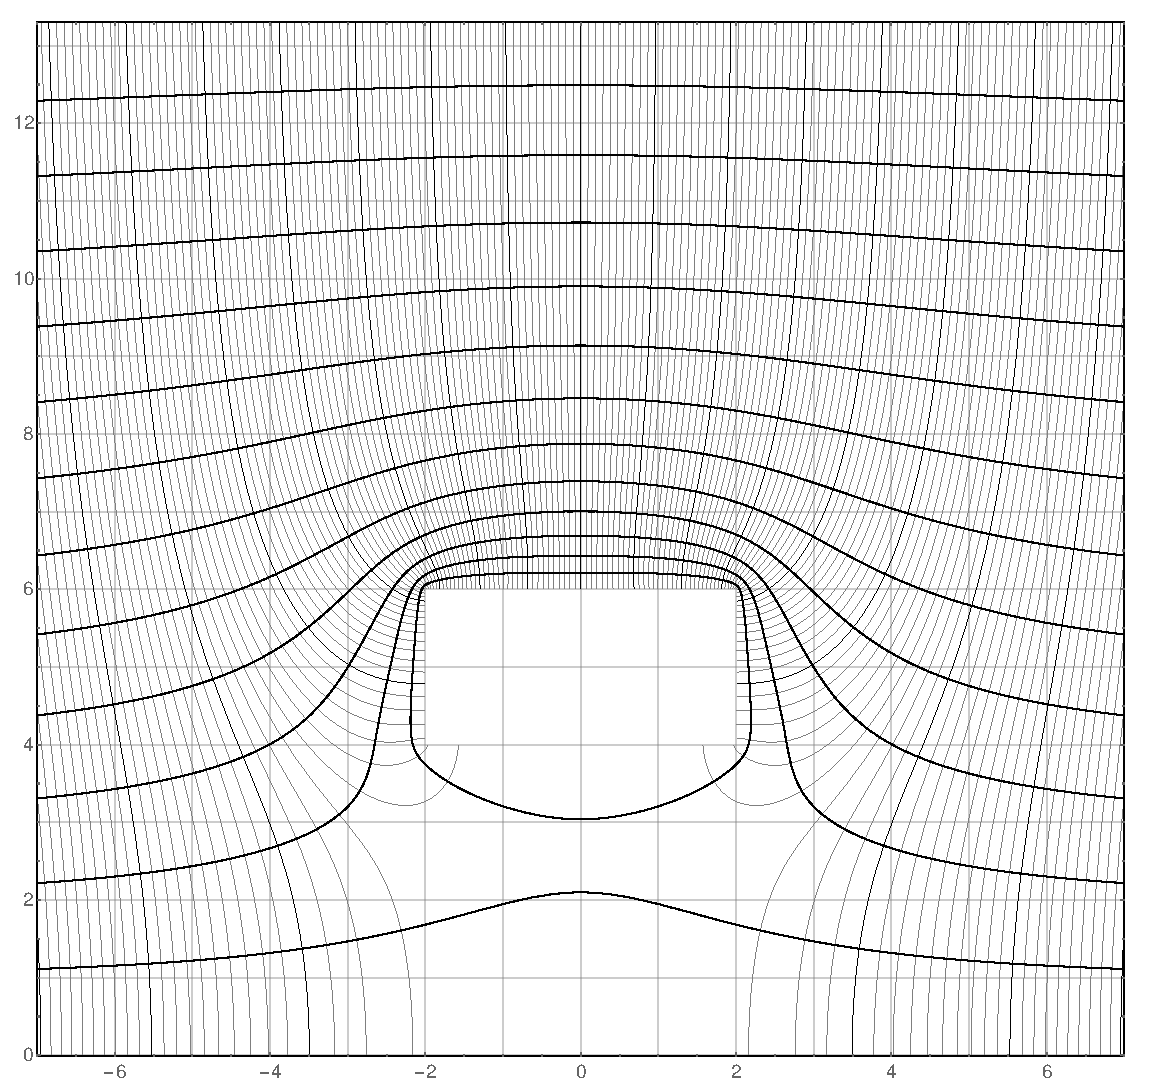
\includegraphics[width=5cm]{uloha3_zadani.pdf}
    \caption{Graf siločar ve svislém řezu procházejícím osou symetrie.}
\end{wrapfigure}

\section*{Úkol 3}

\subsection*{Zadání}
Do homogenního pole se vzdáleností siločar $a$ byl umístěn uzeměný válec o výšce $h=2a$ a poloměru $R=2a$ ve vzdálenosti $H=4a$ od země. Kolikrát nižší by byl náboj indukovaný na elektrodě umístěné na spodní podstavě oproti elektrodě umístěné na horní podstavě? A v jakém vztahu je s intenzitou původního homogenního pole?

\subsection*{Řešení}
Při řešení této úlohy nám bude užitečná veličina $\Phi$ – tok elektrické intenzity $\vec{E}$ plochou $S$ – definovaná jako:
\begin{align*}
    \Phi = \iint_S \vec{E} \cdot \d{\vec{S}}
\end{align*}
Víme, že náboj indukovaný na tělese je přímo úměrný toku elektrické intenzity jeho povrchem:
\begin{align*}
    Q = \frac{\Phi}{\varepsilon_0}
\end{align*}
Elektrody umístíme tak, že zakrývají celou podstavu, tok elektrické intenzity skrz povrch elektrody tak bude rovný toku skrz samotnou podstavu. Víme, že siločáry jsou tradičně značeny tak, aby počet siločar $N$ protínajících nějakou plochu $S$ byl přímo úměrný toku elektrické intenzity přes tuto plochu:
\begin{align*}
    N = \floor{k\Phi}, \;\;\; k = \const{konst.}
\end{align*}
Tato vlastnost platí, pokud jsou siločáry vyobrazeny v trojrozměrném prostoru. Vyobrazíme-li pouze řez úlohou, místo siločar protínajících $S$ ve skutečnosti zobrazujeme siločáry protínající lineární element $\d{S}$. V takovém případě by počet siločar odpovídal $\d{\Phi}$ a bylo by třeba ještě zintegrovat přes plochu.
U grafů axiálně symetrických řezů je ovšem zvykem přenásobit zobrazovanou veličinu faktorem $\pi R$, což efektivně odpovídá zintegrování přes půlkružnici kolem osy. V takovém případě opět platí zmíněný přepočet $N = \floor{k\Phi}$. Budeme předpokládat, že to je i náš případ. Poměr náboje $Q_h$ indukovaného na hroní elektrodě a náboje $Q_s$ indukovaného na spodní elektrodě vypočítáme jednoduše jako poměr počtu siločar protínajících horní a spodní podstavu.

\begin{wrapfigure}{r}{7cm}
    \centering
    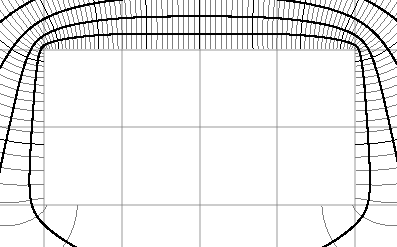
\includegraphics[width=5cm]{uloha3_detail.pdf}
    \caption{Detail siločar kolem válce. Horní podstavu protíná $74$ siločar, spodní $4$.}
\end{wrapfigure}

Platí:
\begin{align*}
    \frac{Q_h}{Q_s} &= \frac{\Phi_h}{\varepsilon_0} \, \frac{\varepsilon_0}{\Phi_s} \approx \frac{N_h}{N_s} = \frac{74}{4} = 18.5
\end{align*}
Citlivost na spodní elektrodě je tedy cca $18.5$-krát nižší.

Nyní stačí vypočítat konstantu úměrnosti $k$ mezi počtem siločar $N$ a tokem intenzity $\Phi$. Víme, že před umístěním válce do homogenního pole $\vec{E}$ byly od sebe tučné siločáry (tj. každá desátá) vzdáleny $a$, to znamená že na plochu $S=a^2$ připadla právě jedna siločára, tedy:
\begin{align*}
    10 = N = k\Phi = k\int_{S=a^2} \vec{E} \cdot \d{\vec{S}} = k a^2 \norm{E} \implies k = \frac{10}{a^2 \norm{E}}
\end{align*}

Na spodní podstavě válce končí 4 siločáry, celkový indukovaný náboj je tam tedy:
\begin{align*}
    \left|Q_s\right|
    = \frac{\Phi}{\varepsilon_0}
    \approx \frac{N_s}{k\varepsilon_0}
    = \frac{4 a^2}{10 \varepsilon_0} \; \norm{E}.
\end{align*}

\end{document}
